\section{Photon Detection System (PD) Overview}
\label{sec:fdsp-pd-ov}
%\metainfo{(Length: TDR=10 pages, TP=3 pages)}

%%%%%%%%%%%%%%%%%%%%%%%%%%%%%%%%%
\subsection{Introduction}
\label{sec:fdsp-pd-intro}
%\todo{\color{blue} Content: Segreto}

The photon detection system is an essential subsystem of the DUNE Single-Phase TPC. The detection of the prompt scintillation light signal, emitted in coincidence with an ionizing event inside the active volume, allows the determination of the time of occurrence of an event of interest a thousand times sooner than charge collected from ionization track and with much higher precision. For physics that is uncorrelated with the accelerator, such as proton decay and neutrinos from supernova burst  this information allows determination of the drift time of the ionizing particles.
Knowledge of the drift time provides localization of the event inside the active volume and provides the ability to correct the measured charge for  effects that depend on the drift path length or for specific locations in the detector if there are non-uniformities.  This correction is important for the reconstruction of the energy deposited by the ionizing event, which otherwise would depend on the drift time and on the purity of the liquid argon. In addition to allowing optimum track reconstruction, scintillation light measured by the system could also be used as trigger and for improved calorimetric measurement in combination with charge measurement.

Liquid argon (LAr) is known to be an abundant scintillator and emits about 40~photons/keV when excited  by minimum ionizing particles\cite{ref:lar-scint}, in absence of external electric fields. The passage of ionizing radiation in LAr produces excitations 
and ionizations of the argon atoms that ultimately results in the formation of the 
\todo{check  correct symbol for excited dimer}excited dimer Ar$^2_*$.  Photon emission proceeds through the de-excitation 
of the lowest lying singlet and triplet excited states, $^{1}\Sigma$ and 
$^{3}\Sigma$ to the dissociative ground state. The de-excitation from the 
$^{1}\Sigma$ state is very fast and has a characteristic time of the order of 
$\tau_{fast}$ $\simeq$ 6 ns. The de-excitation from the $^{3}\Sigma$ state is 
much slower with a characteristic time of $\tau_{slow}$ $\simeq$ 1.3 $\mu$sec, 
since it is forbidden by the selection rules. 
In both decays, photons are emitted in a 10 nm band centered around 127 nm, in 
the Vacuum Ultra Violet (VUV) region of the electromagnetic spectrum.
The relative abundance of the  fast and slow components is related to the ionization density of LAr and 
depends on the ionizing particle: 0.3 for electrons, 1.3 for alpha 
particles and 3. for neutrons. This phenomena is the basis for the  
particle discrimination capabilities of LAr exploited by many 
experiments.

The paradigm for the detection of LAr scintillation light depends on the use of 
chemical wavelength shifters since the currently available commercial (cryogenic) photosensors are not 
directly sensitive to VUV radiation due to the lack of transparency of fused silica and 
glass optical windows. The most widely used wavelength shifter used in 
combination with LAr is Tetra-Phenyl Butadiene (TPB), which absorbs VUV photons 
and re-emits them with a spectrum centered around 430 nm, where most of the 
photosensors have their maximum quantum efficiency for photoconversion. TPB conversion efficiency 
is known to be high, when compared to other wavelength shifters, and 
it is often taken to be 100\%, even though a reliable direct measurement of this 
relevant quantity is not available in the literature. 
In large LAr TPC, it is common to use so-called photon collector systems that attempt to 
collect light from large areas and channel it in an efficient way towards  
photosensors that produce an electrical signal.

%Scintillation light detection plays several important roles in a LAr TPC such as
%a prompt trigger for potential events of interest and to precisely tag the time of the event, $T_0$, which is needed to 
%determine the absolute position of the event inside the active volume.  It may also allow accurate calorimetric measurement of 
%the deposited energy and so contributes to capability of the TPC as a powerful instrument for particle identification.

Table~\ref{tab:pds-req} summarizes the key performance requirements for the photon detection system.
For example, the photon system will provide the timing of events relative to TPC timing, $t_0$, with a 
resolution better than 1 $\mu$sec.  The capability to measure the $t_0$ of non-beam events with deposited 
energy above 200 MeV will allow observation of proton decay and atmospheric neutrinos with high 
efficiency by enabling 3D spatial localization of candidate events. 
There is a minimum light yield requirement is of  0.1 photoelectrons(pe)/MeV for events that occur near the cathode, which is the farthest region from photon collectors that are embedded in the Anode Plane Assembly (APA) described in Chapter\ref{ch:fdsp-apa}. 
A revision of these requirements is being considered in order to better exploit the 
characteristics of LAr scintillation light and to improve the performance of the detector for low energy events such neutrinos from core collapse supernovae.

\fixme{Needs: Performance requirements for the PD system table to expand?}

\begin{dunetable}
[Key performance requirements for the PD system.]
%{p{0.8\textwidth}}
{cc}
{tab:pds-req}
{Highest-level PD performance requirements to achieve the detection efficiency of $90$\% for energy deposit of \SI{> 200}{MeV}} 
Requirement  & Value \\ \toprowrule
Light Yield  & 0.1~pe/MeV for events near the cathode plane  \\ \colhline
Timing Resolution & 1~$\mu$s   \\ \colhline
\end{dunetable}


%\fixme{By the end of the volume, for every requirement listed in this section, there should exist an explanation of how it will be satisfied.}

%\fixme{?? Image of the overall system, indicating its parts. Show how the system fits into the overall detector.}

%\begin{dunefigure}[optional caption for LoF]{fig:figure-label}
%{required full caption (Credit: xyz)}
%\includegraphics[width=0.8\textwidth]{image-filename}
%\end{dunefigure}

%\fixme{Include summary of simulation status? {\color{red}  Szelc/Himmel}}

%%%%%%%%%%%%%%%%%%%%%%%%%%%%%%%%%%%%%
\subsection{Design Considerations}
\label{sec:fdsp-pd-des-consid}
%\todo{\color{blue} Content: Segreto/Warner/Mualem}

The physical dimension of the photon detection (PD) system is constrained by the need to fit within the innermost wire planes of the Anode Plane Assembly (APA) and to be installed into slots in the APA mechanical frame after it is wound (see Section~\ref{sec:fdsp-apa-design}). 
Individual photon detector modules are shaped in the form of thin bars (less than 1 cm thick) with approximate dimensions of 8~cm $\times$ 200~cm. It is currently anticipated that there will be 10 PD modules per APA, for a total of 1500 modules. 

Three different designs of PD modules have been developed and are being 
considered by the Single-Phase Photon Detector Consortium. Two are based on the concept of 
light guides coupled to solid state silicon photomultipliers (SiPM) while the 
third one, namely the ARAPUCA, is functionally a light trap that captures wavelength-shifted photons inside
boxes with highly reflective internal surfaces where they are eventually detected by an
SiPM. Figure~\ref{fig:3dtpc-pd} shows a 3-D model of the Single-Phase TPC with a zoom in to the anode plane where the three candidates photon collector technologies are visible for illustration - in the final detector there will for a single type.

\begin{dunefigure}[3-D model of photon detectors in the APA.]{fig:3dtpc-pd}
{3-D model of photon detectors in the APA. The model on the left shows the full width of the TPC with the configuration APA-CPA-APA-CPA-APA. The right figure shows a zoom in to the top far side of the TPC where three candidates photon collector technologies are visible for illustration - in the final detector there will be a single type.}
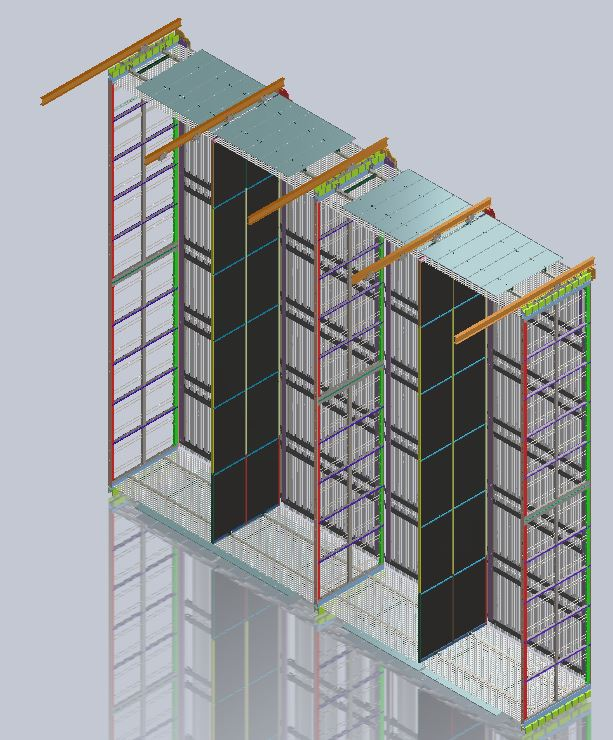
\includegraphics[height=5cm]{pds-dune-sp-tpc-3d.jpg}
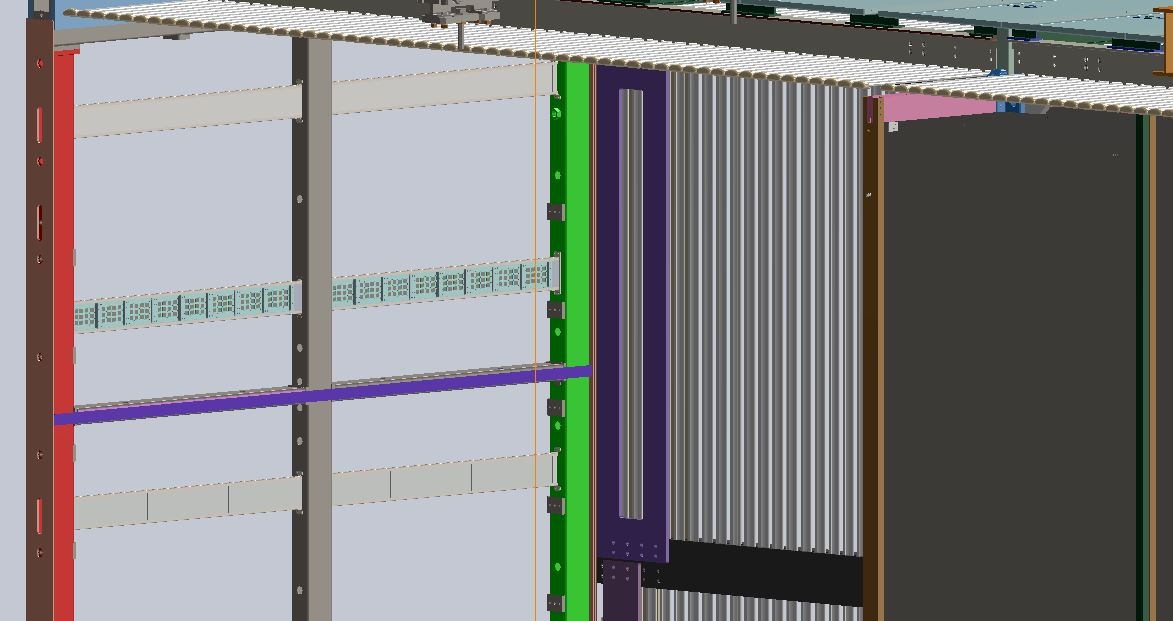
\includegraphics[height=5cm]{pds-dune-sp-tpc-3d-zoom.jpg}
\end{dunefigure}


The dip-coated light guides are pre-treated commercially-cut acrylic slabs dip 
coated with a solution of TPB, acrylic and toluene. When toluene evaporates it 
leaves a thin film of TPB embedded in  acrylic matrix that acts as wavelength 
shifter. A fraction of the light is captured inside the acrylic bar by total 
internal reflection and is detected at one end of the bar by an array of SiPM.

The double-shift light guides are slightly different, since the conversion and 
guiding processes of the photons are decoupled. They are form by a 
radiator plate coated by pure TPB (through a spraying process) that is 
optically coupled to a commercial doped bar that absorbs the blue
light produced by TPB and re-emits it in the green. A fraction of the double-shifted light is 
captured inside the bar by total internal reflections and propagates down the bar until it is incident on an
array of SiPM installed at one end, or possibly both.

The ARAPUCA module is composed of an array of smaller boxes (about 20 per module) 
20) each one acting as a smaller detector. Each box has an optical window made 
by a dichroic filter deposited with two different wavelength shifters, one on 
the external side and another on the internal one, which allows the light to get
inside the box, but not to exit. The internal surface of each box is lined 
with a highly reflective material so that the trapped photon can reflect several 
times before absorption. An array of SiPMs is installed inside the box to detect the light either directly from the window or after some number of bounces. 

The two solid bars designs have been developed over several years and have reached a reasonable level of maturity and reliability. 
Both designs have demonstrated attenuation lengths along the long dimension of the bar of the 
trapped light comparable to the length of the bars themselves, which ensures a reasonable uniformity along the beam direction. Their absolute efficiency has been measured to be in a range between 0.1\% and 0.2\%.
Further  improvements are possible and could come from simple extensions of the design such as installing SiPM at both ends of the bars and coating the smaller sides of the  bars with reflective foils. 
Such improvements provide two important benefits: the efficiency to identify the interaction time 
(and subsequently improve the calorimetric energy resolution of the interaction through drift-distance correction) is substantially improved at all energies; and, perhaps more importantly, the supernova neutrino tagging efficiency is more robust against uncertainty in the final module performance and manufacturing variations between modules once the light collector efficiency. 

Low-energy neutrinos from a galactic core-collapse supernova represent one of the most challenging physics channels for the photon detection system and figure~\ref{fig:pds-sn-eff-simulation} shows the impact of improved PD system performance on neutrino detection efficiency as a function of the energy of the electron produced in the neutrino interaction (this study was done for the double-shift light guide design).  The curve labeled ``standard'' corresponds to the current level of performance and results in an average efficiency for the photon detection system to unambiguously reconstruct the neutrino interaction time to be 30\% at 5~MeV and 70\% at 15~MeV of visible energy. A factor of two increase in PD light yield increases the efficiency at 5~MeV by almost 70\%. 
Since the technology is by now quite mature, the effects of these improvements can be predicted quite well through Monte Carlo simulations; validation of the simulations will come from extensive data from protoDUNE, which will have 29 bars of each type.

\begin{dunefigure}[Neutrino detection efficiency dependence on PD system performance.]
{fig:pds-sn-eff-simulation}
{Preliminary neutrino detection efficiency estimate as a function of the energy of the electron produced in the neutrino interaction for a variety of relative efficiencies of the double-shift light guide detector. The curve marked ``standard'' represents performance of recent prototypes.} 
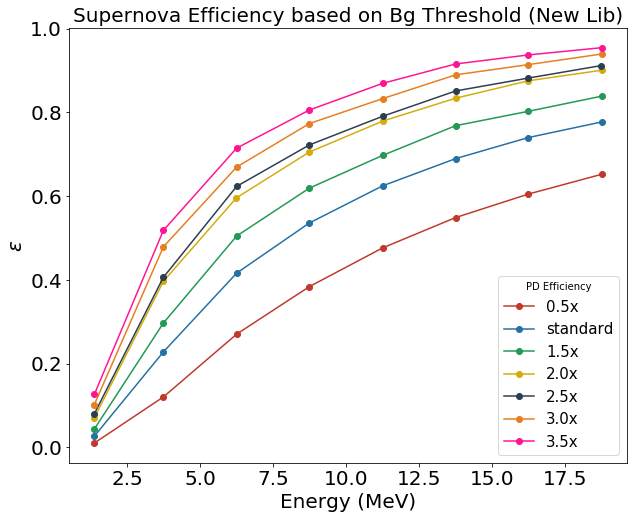
\includegraphics[width=0.5\columnwidth]{pds-sn-eff-simulation.png}
\end{dunefigure}

 
The ARAPUCA concept is quite new since it was proposed for the first time in 2015 and was accepted for the installation in protoDUNE in mid-2016. A series of tests in LAr have been performed with different 
realizations of ARAPUCA devices. These resulted in efficiencies ranging from 
0.4\% to 1.8\%, demonstrating the potential for substantially higher performance than the bar designs. Monte Carlo simulations show that efficiencies at the level of few per cent could be reasonably reached with few modifications to the basic design. 
While the results of the experimental tests are encouraging, for this novel approach a deeper understanding of the optical phenomena involved is needed.

Since the photon detection modules are installed only on the anode plane light collection is not uniform over the entire active volume of the TPC. A possible solution to improve this is to install a reflective foil coated with wavelength shifter on the cathode.
 It would increase the light yield of the detector and could enable calorimetric measurements based on light emitted by the ionizing particles. It may also, through timing cuts, be possible to remove the \Ar39 background that may otherwise cause a huge counting rate for events near  the anode plane. This possibility is under study through Monte Carlo simulations and its mechanical
feasibility is being discussed with the HV Consortium.

The minimal requirements for the light yield of the PD system is of 0.1 
pe/MeV near the cathode, which would allow to efficiently  detect ($>$ 90\%) 
proton decay events (visible energy $>$ 200 MeV). All three designs 
satisfies the minimum requirements according to preliminary Monte Carlo 
studies, but only barely, and there is a consensus inside the Collaboration that a higher 
light yield would be very beneficial for the detection of low energy supernova 
neutrinos so a critical review of the requirements is taking place.

These considerations drive the strategy for the design of the photon collector design and the R\&D program that will 
be carried out before the Technical Design Report (mid-2019). An intense effort 
is underway to explore the possibility that an implementation of the ARAPUCA concept could increase the light yield of the 
detector by a factor ten with respect to the bars; resources (personnel and funding) are being sort by the Consortium to achieve this.  
It is anticipated that by the time of the TDR, the Consortium will present a baseline design for the photon collector and one alternative design for risk mitigation.  

In each photon collector concept, the final stage of converting a visible wavelength photon into an electrical signal will be performed by a silicon photomultipler (SiPM). Our experience with a promising early candidate but that failed in later batches due to an unadvertised change in the device construction has emphasized the importance of a multi-source approach where we are actively engaged with potential vendors to develop a device expressly for cryogenic operation. There are ongoing investigations of a cryogenic SiPM produced by Hamamatsu and by FBK (Fondazione Bruno Kessler, Italy), which developed a device for use in the DarkSide cryogenic experiment.

For prototype development and for protoDUNE, a very capable waveform digitizer has been developed that enables a thorough investigation of the photosensor signals, particularly as we investigate the impact of electrically ganging multiple sensors. The design of the readout electronics for the final system will be strongly influenced by the outcomes of Monte Carlo simulations that are in progress. Of particular interest is the extent to which pulse  shape capabilities are important to maximizing sensitivity to low energy neutrino interactions from supernovae. 
%These consideration will have a role in defining the read-out scheme and the digitization frequency of the signals.  


\subsection{Photon Collection Options Evaluation}
%\todo{\color{blue} Content: Segreto}

The performance of the different photon collection options will be 
evaluated in the facilities available to the Consortium that will allow
relative and absolute measurements to be performed at both room and cryogenic temperatures.
The most comprehensive set of data will come from the fully instrumented modules in the protoDUNE experiment, 
under construction at CERN that will start operations in the last third of 2018.
All  three different photon collector designs are present in protoDUNE: 29 
double-shift guides, 29 dip-coated guides, and two ARAPUCA arrays. The 
presence of the Time Projection Chamber will allow  precise reconstruction
in 3D the track of any ionizing event inside the active volume. The 
matching of the track with the associated light signal will enable an
accurate comparison of the relative detection efficiencies of the different PD 
modules. 
Absolute measurements will be possible depending on the accuracy of the
Monte Carlo simulations of the optical properties of the detector. 
Unfortunately, since some of the optical parameters that 
regulate VUV light propagation in LAr are poorly known, such as Rayleigh 
scattering length, this will influence the precision of the absolute 
measurements. \todo{sounds like we need a plan to measure this somewhere...}

ProtoDUNE will also give the opportunity of performing a longer-term test of full-scale PD modules for the first time. It will be possible to quantify any deterioration in their performance, which will be important input to determining the necessary initial performance level, such as light yield, that will ensure that the minimal requirements are satisfied for the whole life of the DUNE experiment.

An R\&D program will go on in parallel with the protoDUNE operation since 
additonal comparative measurements will be needed, particularly for the newer ARAPUCA concept, before the Technical Design 
Report, which is when a baseline design must be presented.
The TallBo facility at Fermilab will be extremely important for this program. 
It provides a 450 liter capacity cryostat with 56 cm inner diameter and up 
to a 183 cm liquid depth that accommodates  up to three different PD 
modules with dimensions \todo{how different?} close to the real ones.

Other facilities are accessible to the Consortium that will allow testing of
smaller scale prototypes of the modules (or a piece of them). The facilities include: the 
ScENE set-up at Fermilab; the cryogenic facilities at Colorado State 
University and UNICAMP (Brazil); and the optical facilities at Fermilab, 
Indiana University and UNICAMP. These facilities will be valuable for the 
single modules optimization process.

A decision on the light collector technology will be made in February 2019.

\subsection{Scope}
\label{sec:fdsp-pd-scope}
%\todo{\color{blue} Content: Segreto/Warner/Mualem}
The scope of the photon detector (PD) system for the DUNE far detector 
reference design includes design, procurement, fabrication, testing,
 delivery and installation of the following components:
\begin{itemize}
        \item light collection system;
        \item photosensors (silicon photomultipliers);
        \item readout electronics and cabling;
        \item calibration system (tbd);
        \item (TPB-coated foils for the cathode plane (if implemented))
        \item related infrastructures.
\end{itemize}
